\documentclass[1p]{elsarticle_modified}
%\bibliographystyle{elsarticle-num}

%\usepackage[colorlinks]{hyperref}
%\usepackage{abbrmath_seonhwa} %\Abb, \Ascr, \Acal ,\Abf, \Afrak
\usepackage{amsfonts}
\usepackage{amssymb}
\usepackage{amsmath}
\usepackage{amsthm}
\usepackage{scalefnt}
\usepackage{amsbsy}
\usepackage{kotex}
\usepackage{caption}
\usepackage{subfig}
\usepackage{color}
\usepackage{graphicx}
\usepackage{xcolor} %% white, black, red, green, blue, cyan, magenta, yellow
\usepackage{float}
\usepackage{setspace}
\usepackage{hyperref}

\usepackage{tikz}
\usetikzlibrary{arrows}

\usepackage{multirow}
\usepackage{array} % fixed length table
\usepackage{hhline}

%%%%%%%%%%%%%%%%%%%%%
\makeatletter
\renewcommand*\env@matrix[1][\arraystretch]{%
	\edef\arraystretch{#1}%
	\hskip -\arraycolsep
	\let\@ifnextchar\new@ifnextchar
	\array{*\c@MaxMatrixCols c}}
\makeatother %https://tex.stackexchange.com/questions/14071/how-can-i-increase-the-line-spacing-in-a-matrix
%%%%%%%%%%%%%%%

\usepackage[normalem]{ulem}

\newcommand{\msout}[1]{\ifmmode\text{\sout{\ensuremath{#1}}}\else\sout{#1}\fi}
%SOURCE: \msout is \stkout macro in https://tex.stackexchange.com/questions/20609/strikeout-in-math-mode

\newcommand{\cancel}[1]{
	\ifmmode
	{\color{red}\msout{#1}}
	\else
	{\color{red}\sout{#1}}
	\fi
}

\newcommand{\add}[1]{
	{\color{blue}\uwave{#1}}
}

\newcommand{\replace}[2]{
	\ifmmode
	{\color{red}\msout{#1}}{\color{blue}\uwave{#2}}
	\else
	{\color{red}\sout{#1}}{\color{blue}\uwave{#2}}
	\fi
}

\newcommand{\Sol}{\mathcal{S}} %segment
\newcommand{\D}{D} %diagram
\newcommand{\A}{\mathcal{A}} %arc


%%%%%%%%%%%%%%%%%%%%%%%%%%%%%5 test

\def\sl{\operatorname{\textup{SL}}(2,\Cbb)}
\def\psl{\operatorname{\textup{PSL}}(2,\Cbb)}
\def\quan{\mkern 1mu \triangleright \mkern 1mu}

\theoremstyle{definition}
\newtheorem{thm}{Theorem}[section]
\newtheorem{prop}[thm]{Proposition}
\newtheorem{lem}[thm]{Lemma}
\newtheorem{ques}[thm]{Question}
\newtheorem{cor}[thm]{Corollary}
\newtheorem{defn}[thm]{Definition}
\newtheorem{exam}[thm]{Example}
\newtheorem{rmk}[thm]{Remark}
\newtheorem{alg}[thm]{Algorithm}

\newcommand{\I}{\sqrt{-1}}
\begin{document}

%\begin{frontmatter}
%
%\title{Boundary parabolic representations of knots up to 8 crossings}
%
%%% Group authors per affiliation:
%\author{Yunhi Cho} 
%\address{Department of Mathematics, University of Seoul, Seoul, Korea}
%\ead{yhcho@uos.ac.kr}
%
%
%\author{Seonhwa Kim} %\fnref{s_kim}}
%\address{Center for Geometry and Physics, Institute for Basic Science, Pohang, 37673, Korea}
%\ead{ryeona17@ibs.re.kr}
%
%\author{Hyuk Kim}
%\address{Department of Mathematical Sciences, Seoul National University, Seoul 08826, Korea}
%\ead{hyukkim@snu.ac.kr}
%
%\author{Seokbeom Yoon}
%\address{Department of Mathematical Sciences, Seoul National University, Seoul, 08826,  Korea}
%\ead{sbyoon15@snu.ac.kr}
%
%\begin{abstract}
%We find all boundary parabolic representation of knots up to 8 crossings.
%
%\end{abstract}
%\begin{keyword}
%    \MSC[2010] 57M25 
%\end{keyword}
%
%\end{frontmatter}

%\linenumbers
%\tableofcontents
%
\newcommand\colored[1]{\textcolor{white}{\rule[-0.35ex]{0.8em}{1.4ex}}\kern-0.8em\color{red} #1}%
%\newcommand\colored[1]{\textcolor{white}{ #1}\kern-2.17ex	\textcolor{white}{ #1}\kern-1.81ex	\textcolor{white}{ #1}\kern-2.15ex\color{red}#1	}

{\Large $\underline{12a_{0855}~(K12a_{0855})}$}

\setlength{\tabcolsep}{10pt}
\renewcommand{\arraystretch}{1.6}
\vspace{1cm}\begin{tabular}{m{100pt}>{\centering\arraybackslash}m{274pt}}
\multirow{5}{120pt}{
	\centering
	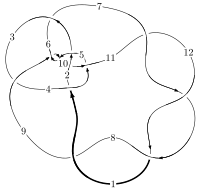
\includegraphics[width=112pt]{../../../GIT/diagram.site/Diagrams/png/1656_12a_0855.png}\\
\ \ \ A knot diagram\footnotemark}&
\allowdisplaybreaks
\textbf{Linearized knot diagam} \\
\cline{2-2}
 &
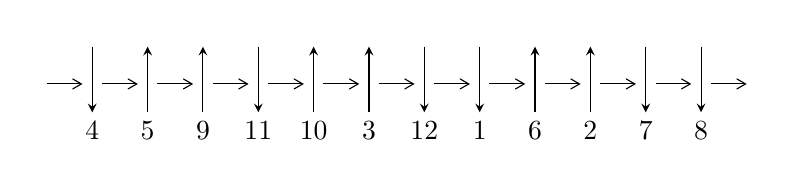
\begin{tikzpicture}[x=20pt, y=17pt]
	% nodes
	\node (C0) at (0, 0) {};
	\node (C1) at (1, 0) {};
	\node (C1U) at (1, +1) {};
	\node (C1D) at (1, -1) {4};

	\node (C2) at (2, 0) {};
	\node (C2U) at (2, +1) {};
	\node (C2D) at (2, -1) {5};

	\node (C3) at (3, 0) {};
	\node (C3U) at (3, +1) {};
	\node (C3D) at (3, -1) {9};

	\node (C4) at (4, 0) {};
	\node (C4U) at (4, +1) {};
	\node (C4D) at (4, -1) {11};

	\node (C5) at (5, 0) {};
	\node (C5U) at (5, +1) {};
	\node (C5D) at (5, -1) {10};

	\node (C6) at (6, 0) {};
	\node (C6U) at (6, +1) {};
	\node (C6D) at (6, -1) {3};

	\node (C7) at (7, 0) {};
	\node (C7U) at (7, +1) {};
	\node (C7D) at (7, -1) {12};

	\node (C8) at (8, 0) {};
	\node (C8U) at (8, +1) {};
	\node (C8D) at (8, -1) {1};

	\node (C9) at (9, 0) {};
	\node (C9U) at (9, +1) {};
	\node (C9D) at (9, -1) {6};

	\node (C10) at (10, 0) {};
	\node (C10U) at (10, +1) {};
	\node (C10D) at (10, -1) {2};

	\node (C11) at (11, 0) {};
	\node (C11U) at (11, +1) {};
	\node (C11D) at (11, -1) {7};

	\node (C12) at (12, 0) {};
	\node (C12U) at (12, +1) {};
	\node (C12D) at (12, -1) {8};
	\node (C13) at (13, 0) {};

	% arrows
	\draw[->,>={angle 60}]
	(C0) edge (C1) (C1) edge (C2) (C2) edge (C3) (C3) edge (C4) (C4) edge (C5) (C5) edge (C6) (C6) edge (C7) (C7) edge (C8) (C8) edge (C9) (C9) edge (C10) (C10) edge (C11) (C11) edge (C12) (C12) edge (C13) ;	\draw[->,>=stealth]
	(C1U) edge (C1D) (C2D) edge (C2U) (C3D) edge (C3U) (C4U) edge (C4D) (C5D) edge (C5U) (C6D) edge (C6U) (C7U) edge (C7D) (C8U) edge (C8D) (C9D) edge (C9U) (C10D) edge (C10U) (C11U) edge (C11D) (C12U) edge (C12D) ;
	\end{tikzpicture} \\
\hhline{~~} \\& 
\textbf{Solving Sequence} \\ \cline{2-2} 
 &
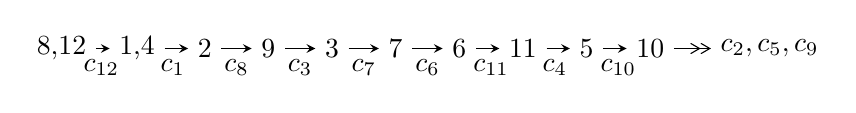
\begin{tikzpicture}[x=23pt, y=7pt]
	% node
	\node (A0) at (-1/8, 0) {8,12};
	\node (A1) at (17/16, 0) {1,4};
	\node (A2) at (17/8, 0) {2};
	\node (A3) at (25/8, 0) {9};
	\node (A4) at (33/8, 0) {3};
	\node (A5) at (41/8, 0) {7};
	\node (A6) at (49/8, 0) {6};
	\node (A7) at (57/8, 0) {11};
	\node (A8) at (65/8, 0) {5};
	\node (A9) at (73/8, 0) {10};
	\node (C1) at (1/2, -1) {$c_{12}$};
	\node (C2) at (13/8, -1) {$c_{1}$};
	\node (C3) at (21/8, -1) {$c_{8}$};
	\node (C4) at (29/8, -1) {$c_{3}$};
	\node (C5) at (37/8, -1) {$c_{7}$};
	\node (C6) at (45/8, -1) {$c_{6}$};
	\node (C7) at (53/8, -1) {$c_{11}$};
	\node (C8) at (61/8, -1) {$c_{4}$};
	\node (C9) at (69/8, -1) {$c_{10}$};
	\node (A10) at (11, 0) {$c_{2},c_{5},c_{9}$};

	% edge
	\draw[->,>=stealth]	
	(A0) edge (A1) (A1) edge (A2) (A2) edge (A3) (A3) edge (A4) (A4) edge (A5) (A5) edge (A6) (A6) edge (A7) (A7) edge (A8) (A8) edge (A9) ;
	\draw[->>,>={angle 60}]	
	(A9) edge (A10);
\end{tikzpicture} \\ 

\end{tabular} \\

\footnotetext{
The image of knot diagram is generated by the software ``\textbf{Draw programme}" developed by Andrew Bartholomew(\url{http://www.layer8.co.uk/maths/draw/index.htm\#Running-draw}), where we modified some parts for our purpose(\url{https://github.com/CATsTAILs/LinksPainter}).
}\phantom \\ \newline 
\centering \textbf{Ideals for irreducible components\footnotemark of $X_{\text{par}}$} 
 
\begin{align*}
I^u_{1}&=\langle 
-2.71973\times10^{150} u^{106}-1.35102\times10^{150} u^{105}+\cdots+2.76810\times10^{149} b+1.95138\times10^{151},\\
\phantom{I^u_{1}}&\phantom{= \langle  }-3.00286\times10^{151} u^{106}-9.93085\times10^{150} u^{105}+\cdots+3.59853\times10^{150} a+1.40666\times10^{152},\\
\phantom{I^u_{1}}&\phantom{= \langle  }u^{107}- u^{106}+\cdots+37 u+13\rangle \\
I^u_{2}&=\langle 
-6 u^{21}+13 u^{20}+\cdots+b-9,\;-8 u^{21}+8 u^{20}+\cdots+a+1,\;u^{22}-14 u^{20}+\cdots-14 u^2+1\rangle \\
\\
\end{align*}
\raggedright * 2 irreducible components of $\dim_{\mathbb{C}}=0$, with total 129 representations.\\
\footnotetext{All coefficients of polynomials are rational numbers. But the coefficients are sometimes approximated in decimal forms when there is not enough margin.}
\newpage
\renewcommand{\arraystretch}{1}
\centering \section*{I. $I^u_{1}= \langle -2.72\times10^{150} u^{106}-1.35\times10^{150} u^{105}+\cdots+2.77\times10^{149} b+1.95\times10^{151},\;-3.00\times10^{151} u^{106}-9.93\times10^{150} u^{105}+\cdots+3.60\times10^{150} a+1.41\times10^{152},\;u^{107}- u^{106}+\cdots+37 u+13 \rangle$}
\flushleft \textbf{(i) Arc colorings}\\
\begin{tabular}{m{7pt} m{180pt} m{7pt} m{180pt} }
\flushright $a_{8}=$&$\begin{pmatrix}0\\u\end{pmatrix}$ \\
\flushright $a_{12}=$&$\begin{pmatrix}1\\0\end{pmatrix}$ \\
\flushright $a_{1}=$&$\begin{pmatrix}1\\u^2\end{pmatrix}$ \\
\flushright $a_{4}=$&$\begin{pmatrix}8.34469 u^{106}+2.75970 u^{105}+\cdots-204.687 u-39.0899\\9.82526 u^{106}+4.88068 u^{105}+\cdots-298.738 u-70.4952\end{pmatrix}$ \\
\flushright $a_{2}=$&$\begin{pmatrix}-18.6646 u^{106}-10.3720 u^{105}+\cdots+546.013 u+156.555\\-31.5456 u^{106}-17.6970 u^{105}+\cdots+941.795 u+275.347\end{pmatrix}$ \\
\flushright $a_{9}=$&$\begin{pmatrix}- u\\- u^3+u\end{pmatrix}$ \\
\flushright $a_{3}=$&$\begin{pmatrix}9.49206 u^{106}+3.47400 u^{105}+\cdots-224.750 u-49.7932\\12.0894 u^{106}+6.28403 u^{105}+\cdots-362.472 u-83.9937\end{pmatrix}$ \\
\flushright $a_{7}=$&$\begin{pmatrix}u\\u\end{pmatrix}$ \\
\flushright $a_{6}=$&$\begin{pmatrix}3.98230 u^{106}+2.01757 u^{105}+\cdots-121.235 u-43.7384\\10.9136 u^{106}+5.89206 u^{105}+\cdots-333.952 u-101.022\end{pmatrix}$ \\
\flushright $a_{11}=$&$\begin{pmatrix}- u^2+1\\- u^2\end{pmatrix}$ \\
\flushright $a_{5}=$&$\begin{pmatrix}14.2838 u^{106}+6.95237 u^{105}+\cdots-388.946 u-108.913\\20.7169 u^{106}+11.3131 u^{105}+\cdots-629.231 u-163.994\end{pmatrix}$ \\
\flushright $a_{10}=$&$\begin{pmatrix}10.9981 u^{106}+8.41827 u^{105}+\cdots-371.282 u-128.867\\18.8426 u^{106}+9.80105 u^{105}+\cdots-556.113 u-162.363\end{pmatrix}$\\&\end{tabular}
\flushleft \textbf{(ii) Obstruction class $= -1$}\\~\\
\flushleft \textbf{(iii) Cusp Shapes $= -7.15694 u^{106}-0.854720 u^{105}+\cdots+135.938 u+10.9433$}\\~\\
\newpage\renewcommand{\arraystretch}{1}
\flushleft \textbf{(iv) u-Polynomials at the component}\newline \\
\begin{tabular}{m{50pt}|m{274pt}}
Crossings & \hspace{64pt}u-Polynomials at each crossing \\
\hline $$\begin{aligned}c_{1}\end{aligned}$$&$\begin{aligned}
&u^{107}+8 u^{106}+\cdots+79200 u-3200
\end{aligned}$\\
\hline $$\begin{aligned}c_{2}\end{aligned}$$&$\begin{aligned}
&u^{107}+8 u^{105}+\cdots-191 u-11
\end{aligned}$\\
\hline $$\begin{aligned}c_{3}\end{aligned}$$&$\begin{aligned}
&u^{107}- u^{106}+\cdots+13886809 u+3405181
\end{aligned}$\\
\hline $$\begin{aligned}c_{4}\end{aligned}$$&$\begin{aligned}
&u^{107}+u^{105}+\cdots+152 u-7
\end{aligned}$\\
\hline $$\begin{aligned}c_{5},c_{9}\end{aligned}$$&$\begin{aligned}
&u^{107}-3 u^{106}+\cdots+22 u+2
\end{aligned}$\\
\hline $$\begin{aligned}c_{6}\end{aligned}$$&$\begin{aligned}
&u^{107}+3 u^{106}+\cdots-604539 u-105767
\end{aligned}$\\
\hline $$\begin{aligned}c_{7},c_{8},c_{11}\\c_{12}\end{aligned}$$&$\begin{aligned}
&u^{107}- u^{106}+\cdots+37 u+13
\end{aligned}$\\
\hline $$\begin{aligned}c_{10}\end{aligned}$$&$\begin{aligned}
&u^{107}-6 u^{106}+\cdots+5194 u-4049
\end{aligned}$\\
\hline
\end{tabular}\\~\\
\newpage\renewcommand{\arraystretch}{1}
\flushleft \textbf{(v) Riley Polynomials at the component}\newline \\
\begin{tabular}{m{50pt}|m{274pt}}
Crossings & \hspace{64pt}Riley Polynomials at each crossing \\
\hline $$\begin{aligned}c_{1}\end{aligned}$$&$\begin{aligned}
&y^{107}-40 y^{106}+\cdots+1928422400 y-10240000
\end{aligned}$\\
\hline $$\begin{aligned}c_{2}\end{aligned}$$&$\begin{aligned}
&y^{107}+16 y^{106}+\cdots-7937 y-121
\end{aligned}$\\
\hline $$\begin{aligned}c_{3}\end{aligned}$$&$\begin{aligned}
&y^{107}+47 y^{106}+\cdots-467129995532381 y-11595257642761
\end{aligned}$\\
\hline $$\begin{aligned}c_{4}\end{aligned}$$&$\begin{aligned}
&y^{107}+2 y^{106}+\cdots+5576 y-49
\end{aligned}$\\
\hline $$\begin{aligned}c_{5},c_{9}\end{aligned}$$&$\begin{aligned}
&y^{107}+81 y^{106}+\cdots+1044 y-4
\end{aligned}$\\
\hline $$\begin{aligned}c_{6}\end{aligned}$$&$\begin{aligned}
&y^{107}+31 y^{106}+\cdots-214514614873 y-11186658289
\end{aligned}$\\
\hline $$\begin{aligned}c_{7},c_{8},c_{11}\\c_{12}\end{aligned}$$&$\begin{aligned}
&y^{107}-129 y^{106}+\cdots+5711 y-169
\end{aligned}$\\
\hline $$\begin{aligned}c_{10}\end{aligned}$$&$\begin{aligned}
&y^{107}+26 y^{106}+\cdots-541032280 y-16394401
\end{aligned}$\\
\hline
\end{tabular}\\~\\
\newpage\flushleft \textbf{(vi) Complex Volumes and Cusp Shapes}
$$\begin{array}{c|c|c}  
\text{Solutions to }I^u_{1}& \I (\text{vol} + \sqrt{-1}CS) & \text{Cusp shape}\\
 \hline 
\begin{aligned}
u &= -0.826655 + 0.568633 I \\
a &= \phantom{-}1.24553 + 0.76935 I \\
b &= -0.239026 - 0.064980 I\end{aligned}
 & -6.3082 + 14.5498 I & \phantom{-0.000000 } 0 \\ \hline\begin{aligned}
u &= -0.826655 - 0.568633 I \\
a &= \phantom{-}1.24553 - 0.76935 I \\
b &= -0.239026 + 0.064980 I\end{aligned}
 & -6.3082 - 14.5498 I & \phantom{-0.000000 } 0 \\ \hline\begin{aligned}
u &= \phantom{-}0.826318 + 0.570704 I \\
a &= \phantom{-}1.162670 - 0.663776 I \\
b &= -0.166220 + 0.227032 I\end{aligned}
 & -1.31108 - 8.80416 I & \phantom{-0.000000 } 0 \\ \hline\begin{aligned}
u &= \phantom{-}0.826318 - 0.570704 I \\
a &= \phantom{-}1.162670 + 0.663776 I \\
b &= -0.166220 - 0.227032 I\end{aligned}
 & -1.31108 + 8.80416 I & \phantom{-0.000000 } 0 \\ \hline\begin{aligned}
u &= -0.952140 + 0.249038 I \\
a &= -1.066520 + 0.168283 I \\
b &= \phantom{-}0.474150 - 0.262800 I\end{aligned}
 & -6.05633 + 4.48287 I & \phantom{-0.000000 } 0 \\ \hline\begin{aligned}
u &= -0.952140 - 0.249038 I \\
a &= -1.066520 - 0.168283 I \\
b &= \phantom{-}0.474150 + 0.262800 I\end{aligned}
 & -6.05633 - 4.48287 I & \phantom{-0.000000 } 0 \\ \hline\begin{aligned}
u &= -0.755159 + 0.631053 I \\
a &= \phantom{-}0.862027 + 0.687544 I \\
b &= -0.465536 - 0.607906 I\end{aligned}
 & -5.17350 + 1.52550 I & \phantom{-0.000000 } 0 \\ \hline\begin{aligned}
u &= -0.755159 - 0.631053 I \\
a &= \phantom{-}0.862027 - 0.687544 I \\
b &= -0.465536 + 0.607906 I\end{aligned}
 & -5.17350 - 1.52550 I & \phantom{-0.000000 } 0 \\ \hline\begin{aligned}
u &= \phantom{-}0.894153 + 0.343291 I \\
a &= \phantom{-}1.01314 - 1.38448 I \\
b &= \phantom{-}0.664382 - 0.567740 I\end{aligned}
 & -7.12672 - 5.99311 I & \phantom{-0.000000 } 0 \\ \hline\begin{aligned}
u &= \phantom{-}0.894153 - 0.343291 I \\
a &= \phantom{-}1.01314 + 1.38448 I \\
b &= \phantom{-}0.664382 + 0.567740 I\end{aligned}
 & -7.12672 + 5.99311 I & \phantom{-0.000000 } 0\\
 \hline 
 \end{array}$$\newpage$$\begin{array}{c|c|c}  
\text{Solutions to }I^u_{1}& \I (\text{vol} + \sqrt{-1}CS) & \text{Cusp shape}\\
 \hline 
\begin{aligned}
u &= \phantom{-}0.930030 + 0.515744 I \\
a &= -0.687057 + 0.215263 I \\
b &= \phantom{-}0.130481 + 0.299587 I\end{aligned}
 & -3.25087 - 5.76442 I & \phantom{-0.000000 } 0 \\ \hline\begin{aligned}
u &= \phantom{-}0.930030 - 0.515744 I \\
a &= -0.687057 - 0.215263 I \\
b &= \phantom{-}0.130481 - 0.299587 I\end{aligned}
 & -3.25087 + 5.76442 I & \phantom{-0.000000 } 0 \\ \hline\begin{aligned}
u &= -0.743000 + 0.562440 I \\
a &= -0.380844 - 0.646698 I \\
b &= \phantom{-}0.201098 - 0.163543 I\end{aligned}
 & -1.32303 + 2.45240 I & \phantom{-0.000000 } 0 \\ \hline\begin{aligned}
u &= -0.743000 - 0.562440 I \\
a &= -0.380844 + 0.646698 I \\
b &= \phantom{-}0.201098 + 0.163543 I\end{aligned}
 & -1.32303 - 2.45240 I & \phantom{-0.000000 } 0 \\ \hline\begin{aligned}
u &= \phantom{-}1.005200 + 0.454195 I \\
a &= \phantom{-}0.381919 - 1.027960 I \\
b &= \phantom{-}0.228876 - 0.248331 I\end{aligned}
 & -7.48788 + 5.95732 I & \phantom{-0.000000 } 0 \\ \hline\begin{aligned}
u &= \phantom{-}1.005200 - 0.454195 I \\
a &= \phantom{-}0.381919 + 1.027960 I \\
b &= \phantom{-}0.228876 + 0.248331 I\end{aligned}
 & -7.48788 - 5.95732 I & \phantom{-0.000000 } 0 \\ \hline\begin{aligned}
u &= -1.038100 + 0.394850 I \\
a &= \phantom{-}0.710898 + 0.790455 I \\
b &= \phantom{-}0.490308 + 0.067744 I\end{aligned}
 & -2.72871 - 0.23789 I & \phantom{-0.000000 } 0 \\ \hline\begin{aligned}
u &= -1.038100 - 0.394850 I \\
a &= \phantom{-}0.710898 - 0.790455 I \\
b &= \phantom{-}0.490308 - 0.067744 I\end{aligned}
 & -2.72871 + 0.23789 I & \phantom{-0.000000 } 0 \\ \hline\begin{aligned}
u &= \phantom{-}0.800127 + 0.353920 I \\
a &= -1.42217 + 0.40443 I \\
b &= \phantom{-}0.177923 + 0.234950 I\end{aligned}
 & -2.76423 - 4.13132 I & \phantom{-0.000000 } 0 \\ \hline\begin{aligned}
u &= \phantom{-}0.800127 - 0.353920 I \\
a &= -1.42217 - 0.40443 I \\
b &= \phantom{-}0.177923 - 0.234950 I\end{aligned}
 & -2.76423 + 4.13132 I & \phantom{-0.000000 } 0\\
 \hline 
 \end{array}$$\newpage$$\begin{array}{c|c|c}  
\text{Solutions to }I^u_{1}& \I (\text{vol} + \sqrt{-1}CS) & \text{Cusp shape}\\
 \hline 
\begin{aligned}
u &= -1.128530 + 0.019920 I \\
a &= \phantom{-}0.973765 - 0.309888 I \\
b &= \phantom{-}0.746272 - 0.341276 I\end{aligned}
 & -2.30327 + 0.08679 I & \phantom{-0.000000 } 0 \\ \hline\begin{aligned}
u &= -1.128530 - 0.019920 I \\
a &= \phantom{-}0.973765 + 0.309888 I \\
b &= \phantom{-}0.746272 + 0.341276 I\end{aligned}
 & -2.30327 - 0.08679 I & \phantom{-0.000000 } 0 \\ \hline\begin{aligned}
u &= -0.745803 + 0.416141 I \\
a &= -1.57506 - 1.14608 I \\
b &= \phantom{-}0.125676 - 0.466047 I\end{aligned}
 & -6.27522 + 5.09865 I & \phantom{-0.000000 } 0 \\ \hline\begin{aligned}
u &= -0.745803 - 0.416141 I \\
a &= -1.57506 + 1.14608 I \\
b &= \phantom{-}0.125676 + 0.466047 I\end{aligned}
 & -6.27522 - 5.09865 I & \phantom{-0.000000 } 0 \\ \hline\begin{aligned}
u &= -0.270313 + 0.732731 I \\
a &= \phantom{-}0.372324 - 0.269561 I \\
b &= \phantom{-}0.0940821 - 0.0178112 I\end{aligned}
 & \phantom{-}0.11533 + 1.88710 I & \phantom{-0.000000 } 0 \\ \hline\begin{aligned}
u &= -0.270313 - 0.732731 I \\
a &= \phantom{-}0.372324 + 0.269561 I \\
b &= \phantom{-}0.0940821 + 0.0178112 I\end{aligned}
 & \phantom{-}0.11533 - 1.88710 I & \phantom{-0.000000 } 0 \\ \hline\begin{aligned}
u &= \phantom{-}0.108521 + 0.773022 I \\
a &= -0.193997 - 0.092772 I \\
b &= -0.830652 + 0.465756 I\end{aligned}
 & \phantom{-}0.87016 + 4.32926 I & \phantom{-0.000000 } 0 \\ \hline\begin{aligned}
u &= \phantom{-}0.108521 - 0.773022 I \\
a &= -0.193997 + 0.092772 I \\
b &= -0.830652 - 0.465756 I\end{aligned}
 & \phantom{-}0.87016 - 4.32926 I & \phantom{-0.000000 } 0 \\ \hline\begin{aligned}
u &= \phantom{-}0.678973 + 0.383166 I \\
a &= -0.43360 + 1.55662 I \\
b &= \phantom{-}0.516580 + 0.114540 I\end{aligned}
 & -6.38076 - 0.82493 I & \phantom{-0.000000 } 0 \\ \hline\begin{aligned}
u &= \phantom{-}0.678973 - 0.383166 I \\
a &= -0.43360 - 1.55662 I \\
b &= \phantom{-}0.516580 - 0.114540 I\end{aligned}
 & -6.38076 + 0.82493 I & \phantom{-0.000000 } 0\\
 \hline 
 \end{array}$$\newpage$$\begin{array}{c|c|c}  
\text{Solutions to }I^u_{1}& \I (\text{vol} + \sqrt{-1}CS) & \text{Cusp shape}\\
 \hline 
\begin{aligned}
u &= -0.094171 + 0.764360 I \\
a &= -0.488244 + 0.039795 I \\
b &= -0.879858 - 0.577966 I\end{aligned}
 & -4.09729 - 10.11170 I & \phantom{-0.000000 } 0 \\ \hline\begin{aligned}
u &= -0.094171 - 0.764360 I \\
a &= -0.488244 - 0.039795 I \\
b &= -0.879858 + 0.577966 I\end{aligned}
 & -4.09729 + 10.11170 I & \phantom{-0.000000 } 0 \\ \hline\begin{aligned}
u &= \phantom{-}0.388819 + 0.579837 I \\
a &= \phantom{-}0.934771 + 0.492384 I \\
b &= \phantom{-}0.264435 + 0.628142 I\end{aligned}
 & -1.72461 - 1.96082 I & \phantom{-0.000000 -}0. + 4.69802 I \\ \hline\begin{aligned}
u &= \phantom{-}0.388819 - 0.579837 I \\
a &= \phantom{-}0.934771 - 0.492384 I \\
b &= \phantom{-}0.264435 - 0.628142 I\end{aligned}
 & -1.72461 + 1.96082 I & \phantom{-0.000000 } 0. - 4.69802 I \\ \hline\begin{aligned}
u &= -0.575845 + 0.393068 I \\
a &= \phantom{-}1.087690 + 0.019654 I \\
b &= \phantom{-}0.161817 - 0.321184 I\end{aligned}
 & -1.36848 + 1.44447 I & -2.91055 - 4.72054 I \\ \hline\begin{aligned}
u &= -0.575845 - 0.393068 I \\
a &= \phantom{-}1.087690 - 0.019654 I \\
b &= \phantom{-}0.161817 + 0.321184 I\end{aligned}
 & -1.36848 - 1.44447 I & -2.91055 + 4.72054 I \\ \hline\begin{aligned}
u &= -0.213091 + 0.648713 I \\
a &= \phantom{-}0.045157 + 0.915947 I \\
b &= -0.892764 - 0.421227 I\end{aligned}
 & -3.70568 + 2.84318 I & -4.74637 - 7.45487 I \\ \hline\begin{aligned}
u &= -0.213091 - 0.648713 I \\
a &= \phantom{-}0.045157 - 0.915947 I \\
b &= -0.892764 + 0.421227 I\end{aligned}
 & -3.70568 - 2.84318 I & -4.74637 + 7.45487 I \\ \hline\begin{aligned}
u &= \phantom{-}0.666901 + 0.009105 I \\
a &= -1.66225 + 1.18426 I \\
b &= \phantom{-}0.657173 + 0.836987 I\end{aligned}
 & -5.89625 - 0.14698 I & -10.30166 - 0.10648 I \\ \hline\begin{aligned}
u &= \phantom{-}0.666901 - 0.009105 I \\
a &= -1.66225 - 1.18426 I \\
b &= \phantom{-}0.657173 - 0.836987 I\end{aligned}
 & -5.89625 + 0.14698 I & -10.30166 + 0.10648 I\\
 \hline 
 \end{array}$$\newpage$$\begin{array}{c|c|c}  
\text{Solutions to }I^u_{1}& \I (\text{vol} + \sqrt{-1}CS) & \text{Cusp shape}\\
 \hline 
\begin{aligned}
u &= \phantom{-}0.596289 + 0.285850 I \\
a &= -2.90410 + 0.32830 I \\
b &= -0.369695 - 0.037100 I\end{aligned}
 & -2.18570 - 6.38810 I & -3.13881 + 11.21686 I \\ \hline\begin{aligned}
u &= \phantom{-}0.596289 - 0.285850 I \\
a &= -2.90410 - 0.32830 I \\
b &= -0.369695 + 0.037100 I\end{aligned}
 & -2.18570 + 6.38810 I & -3.13881 - 11.21686 I \\ \hline\begin{aligned}
u &= -0.131185 + 0.631680 I \\
a &= \phantom{-}0.488911 - 0.353615 I \\
b &= -0.012361 - 0.410523 I\end{aligned}
 & -0.03169 + 1.79207 I & \phantom{-}3.57282 - 1.79656 I \\ \hline\begin{aligned}
u &= -0.131185 - 0.631680 I \\
a &= \phantom{-}0.488911 + 0.353615 I \\
b &= -0.012361 + 0.410523 I\end{aligned}
 & -0.03169 - 1.79207 I & \phantom{-}3.57282 + 1.79656 I \\ \hline\begin{aligned}
u &= -0.592482 + 0.205435 I \\
a &= -0.609364 + 0.716647 I \\
b &= -0.17971 - 1.60405 I\end{aligned}
 & -2.59941 + 5.79531 I & -3.45472 - 10.54157 I \\ \hline\begin{aligned}
u &= -0.592482 - 0.205435 I \\
a &= -0.609364 - 0.716647 I \\
b &= -0.17971 + 1.60405 I\end{aligned}
 & -2.59941 - 5.79531 I & -3.45472 + 10.54157 I \\ \hline\begin{aligned}
u &= -0.606784 + 0.152467 I \\
a &= -2.90825 + 1.03073 I \\
b &= -0.226483 + 0.599261 I\end{aligned}
 & \phantom{-}0.14553 + 2.03996 I & -5.55929 - 6.74240 I \\ \hline\begin{aligned}
u &= -0.606784 - 0.152467 I \\
a &= -2.90825 - 1.03073 I \\
b &= -0.226483 - 0.599261 I\end{aligned}
 & \phantom{-}0.14553 - 2.03996 I & -5.55929 + 6.74240 I \\ \hline\begin{aligned}
u &= \phantom{-}1.367050 + 0.286263 I \\
a &= \phantom{-}0.127328 + 0.290641 I \\
b &= -0.059407 + 0.653964 I\end{aligned}
 & -5.04557 - 5.52068 I & \phantom{-0.000000 } 0 \\ \hline\begin{aligned}
u &= \phantom{-}1.367050 - 0.286263 I \\
a &= \phantom{-}0.127328 - 0.290641 I \\
b &= -0.059407 - 0.653964 I\end{aligned}
 & -5.04557 + 5.52068 I & \phantom{-0.000000 } 0\\
 \hline 
 \end{array}$$\newpage$$\begin{array}{c|c|c}  
\text{Solutions to }I^u_{1}& \I (\text{vol} + \sqrt{-1}CS) & \text{Cusp shape}\\
 \hline 
\begin{aligned}
u &= \phantom{-}0.523351 + 0.282998 I \\
a &= \phantom{-}0.075777 - 0.409242 I \\
b &= -0.227408 + 1.069820 I\end{aligned}
 & \phantom{-}1.37793 - 2.66689 I & \phantom{-}3.20906 + 9.66179 I \\ \hline\begin{aligned}
u &= \phantom{-}0.523351 - 0.282998 I \\
a &= \phantom{-}0.075777 + 0.409242 I \\
b &= -0.227408 - 1.069820 I\end{aligned}
 & \phantom{-}1.37793 + 2.66689 I & \phantom{-}3.20906 - 9.66179 I \\ \hline\begin{aligned}
u &= -0.054601 + 0.509352 I \\
a &= \phantom{-}1.305150 + 0.511862 I \\
b &= \phantom{-}0.868600 + 0.411289 I\end{aligned}
 & -4.27961 - 1.91423 I & -5.19806 + 3.02668 I \\ \hline\begin{aligned}
u &= -0.054601 - 0.509352 I \\
a &= \phantom{-}1.305150 - 0.511862 I \\
b &= \phantom{-}0.868600 - 0.411289 I\end{aligned}
 & -4.27961 + 1.91423 I & -5.19806 - 3.02668 I \\ \hline\begin{aligned}
u &= -1.51066 + 0.01600 I \\
a &= \phantom{-}0.418299 + 0.263996 I \\
b &= \phantom{-}1.252000 - 0.484762 I\end{aligned}
 & -7.30569 + 3.49955 I & \phantom{-0.000000 } 0 \\ \hline\begin{aligned}
u &= -1.51066 - 0.01600 I \\
a &= \phantom{-}0.418299 - 0.263996 I \\
b &= \phantom{-}1.252000 + 0.484762 I\end{aligned}
 & -7.30569 - 3.49955 I & \phantom{-0.000000 } 0 \\ \hline\begin{aligned}
u &= -0.130339 + 0.458302 I \\
a &= \phantom{-}0.726225 - 0.442383 I \\
b &= \phantom{-}0.347372 - 0.529775 I\end{aligned}
 & -0.127455 + 1.387300 I & -1.33789 - 2.89703 I \\ \hline\begin{aligned}
u &= -0.130339 - 0.458302 I \\
a &= \phantom{-}0.726225 + 0.442383 I \\
b &= \phantom{-}0.347372 + 0.529775 I\end{aligned}
 & -0.127455 - 1.387300 I & -1.33789 + 2.89703 I \\ \hline\begin{aligned}
u &= -0.453754 + 0.108285 I \\
a &= -0.04965 + 1.64879 I \\
b &= \phantom{-}0.540457 + 1.147730 I\end{aligned}
 & \phantom{-}0.643121 - 0.885450 I & -1.73889 - 3.55551 I \\ \hline\begin{aligned}
u &= -0.453754 - 0.108285 I \\
a &= -0.04965 - 1.64879 I \\
b &= \phantom{-}0.540457 - 1.147730 I\end{aligned}
 & \phantom{-}0.643121 + 0.885450 I & -1.73889 + 3.55551 I\\
 \hline 
 \end{array}$$\newpage$$\begin{array}{c|c|c}  
\text{Solutions to }I^u_{1}& \I (\text{vol} + \sqrt{-1}CS) & \text{Cusp shape}\\
 \hline 
\begin{aligned}
u &= \phantom{-}1.53593 + 0.00041 I \\
a &= \phantom{-}1.94990 + 1.21251 I \\
b &= \phantom{-}3.38519 + 1.90248 I\end{aligned}
 & -8.57444 + 3.57156 I & \phantom{-0.000000 } 0 \\ \hline\begin{aligned}
u &= \phantom{-}1.53593 - 0.00041 I \\
a &= \phantom{-}1.94990 - 1.21251 I \\
b &= \phantom{-}3.38519 - 1.90248 I\end{aligned}
 & -8.57444 - 3.57156 I & \phantom{-0.000000 } 0 \\ \hline\begin{aligned}
u &= -0.388804 + 0.226078 I \\
a &= \phantom{-}3.22669 - 1.04826 I \\
b &= -0.440064 + 0.555353 I\end{aligned}
 & -2.04622 - 4.07547 I & -0.50699 - 3.20827 I \\ \hline\begin{aligned}
u &= -0.388804 - 0.226078 I \\
a &= \phantom{-}3.22669 + 1.04826 I \\
b &= -0.440064 - 0.555353 I\end{aligned}
 & -2.04622 + 4.07547 I & -0.50699 + 3.20827 I \\ \hline\begin{aligned}
u &= \phantom{-}0.333256 + 0.298984 I \\
a &= \phantom{-}2.14138 - 0.52844 I \\
b &= -0.471791 - 0.066122 I\end{aligned}
 & \phantom{-}1.86436 + 0.38575 I & \phantom{-}5.67353 + 2.84630 I \\ \hline\begin{aligned}
u &= \phantom{-}0.333256 - 0.298984 I \\
a &= \phantom{-}2.14138 + 0.52844 I \\
b &= -0.471791 + 0.066122 I\end{aligned}
 & \phantom{-}1.86436 - 0.38575 I & \phantom{-}5.67353 - 2.84630 I \\ \hline\begin{aligned}
u &= -1.55441\phantom{ +0.000000I} \\
a &= \phantom{-}2.20352\phantom{ +0.000000I} \\
b &= \phantom{-}3.90175\phantom{ +0.000000I}\end{aligned}
 & -4.55561\phantom{ +0.000000I} & \phantom{-0.000000 } 0 \\ \hline\begin{aligned}
u &= \phantom{-}0.310054 + 0.318457 I \\
a &= \phantom{-}0.84539 - 1.42016 I \\
b &= \phantom{-}0.743246 - 0.990318 I\end{aligned}
 & -1.38392 + 4.09651 I & \phantom{-}1.050672 - 0.014571 I \\ \hline\begin{aligned}
u &= \phantom{-}0.310054 - 0.318457 I \\
a &= \phantom{-}0.84539 + 1.42016 I \\
b &= \phantom{-}0.743246 + 0.990318 I\end{aligned}
 & -1.38392 - 4.09651 I & \phantom{-}1.050672 + 0.014571 I \\ \hline\begin{aligned}
u &= \phantom{-}1.55646 + 0.06741 I \\
a &= \phantom{-}1.093070 - 0.275160 I \\
b &= \phantom{-}2.35045 - 0.12880 I\end{aligned}
 & -8.49647 - 2.94856 I & \phantom{-0.000000 } 0\\
 \hline 
 \end{array}$$\newpage$$\begin{array}{c|c|c}  
\text{Solutions to }I^u_{1}& \I (\text{vol} + \sqrt{-1}CS) & \text{Cusp shape}\\
 \hline 
\begin{aligned}
u &= \phantom{-}1.55646 - 0.06741 I \\
a &= \phantom{-}1.093070 + 0.275160 I \\
b &= \phantom{-}2.35045 + 0.12880 I\end{aligned}
 & -8.49647 + 2.94856 I & \phantom{-0.000000 } 0 \\ \hline\begin{aligned}
u &= -1.57542 + 0.04875 I \\
a &= \phantom{-}0.301319 + 1.218030 I \\
b &= \phantom{-}0.65085 + 1.32300 I\end{aligned}
 & -5.85412 + 3.68887 I & \phantom{-0.000000 } 0 \\ \hline\begin{aligned}
u &= -1.57542 - 0.04875 I \\
a &= \phantom{-}0.301319 - 1.218030 I \\
b &= \phantom{-}0.65085 - 1.32300 I\end{aligned}
 & -5.85412 - 3.68887 I & \phantom{-0.000000 } 0 \\ \hline\begin{aligned}
u &= \phantom{-}1.57646 + 0.00668 I \\
a &= -0.315882 + 0.122479 I \\
b &= -0.407087 - 0.879129 I\end{aligned}
 & -6.50230 + 0.63577 I & \phantom{-0.000000 } 0 \\ \hline\begin{aligned}
u &= \phantom{-}1.57646 - 0.00668 I \\
a &= -0.315882 - 0.122479 I \\
b &= -0.407087 + 0.879129 I\end{aligned}
 & -6.50230 - 0.63577 I & \phantom{-0.000000 } 0 \\ \hline\begin{aligned}
u &= -1.59602 + 0.06317 I \\
a &= -2.18540 + 0.44125 I \\
b &= -4.64805 + 0.94344 I\end{aligned}
 & -9.77380 + 7.56844 I & \phantom{-0.000000 } 0 \\ \hline\begin{aligned}
u &= -1.59602 - 0.06317 I \\
a &= -2.18540 - 0.44125 I \\
b &= -4.64805 - 0.94344 I\end{aligned}
 & -9.77380 - 7.56844 I & \phantom{-0.000000 } 0 \\ \hline\begin{aligned}
u &= \phantom{-}1.60196 + 0.04672 I \\
a &= -0.16909 - 1.99689 I \\
b &= -0.25317 - 2.61736 I\end{aligned}
 & -10.26230 - 6.65235 I & \phantom{-0.000000 } 0 \\ \hline\begin{aligned}
u &= \phantom{-}1.60196 - 0.04672 I \\
a &= -0.16909 + 1.99689 I \\
b &= -0.25317 + 2.61736 I\end{aligned}
 & -10.26230 + 6.65235 I & \phantom{-0.000000 } 0 \\ \hline\begin{aligned}
u &= -1.60126 + 0.12605 I \\
a &= -1.69718 - 0.94538 I \\
b &= -2.98785 - 1.76643 I\end{aligned}
 & -14.1458 + 2.7966 I & \phantom{-0.000000 } 0\\
 \hline 
 \end{array}$$\newpage$$\begin{array}{c|c|c}  
\text{Solutions to }I^u_{1}& \I (\text{vol} + \sqrt{-1}CS) & \text{Cusp shape}\\
 \hline 
\begin{aligned}
u &= -1.60126 - 0.12605 I \\
a &= -1.69718 + 0.94538 I \\
b &= -2.98785 + 1.76643 I\end{aligned}
 & -14.1458 - 2.7966 I & \phantom{-0.000000 } 0 \\ \hline\begin{aligned}
u &= \phantom{-}1.60618 + 0.03641 I \\
a &= -2.01459 - 0.54776 I \\
b &= -4.24925 - 1.61665 I\end{aligned}
 & -7.59927 - 2.69628 I & \phantom{-0.000000 } 0 \\ \hline\begin{aligned}
u &= \phantom{-}1.60618 - 0.03641 I \\
a &= -2.01459 + 0.54776 I \\
b &= -4.24925 + 1.61665 I\end{aligned}
 & -7.59927 + 2.69628 I & \phantom{-0.000000 } 0 \\ \hline\begin{aligned}
u &= -1.62630 + 0.00862 I \\
a &= -1.91576 - 0.09707 I \\
b &= -3.47477 + 0.56297 I\end{aligned}
 & -13.98410 - 0.07693 I & \phantom{-0.000000 } 0 \\ \hline\begin{aligned}
u &= -1.62630 - 0.00862 I \\
a &= -1.91576 + 0.09707 I \\
b &= -3.47477 - 0.56297 I\end{aligned}
 & -13.98410 + 0.07693 I & \phantom{-0.000000 } 0 \\ \hline\begin{aligned}
u &= \phantom{-}1.62253 + 0.11727 I \\
a &= -2.33065 - 0.05749 I \\
b &= -4.37343 + 0.19986 I\end{aligned}
 & -14.3859 - 7.1012 I & \phantom{-0.000000 } 0 \\ \hline\begin{aligned}
u &= \phantom{-}1.62253 - 0.11727 I \\
a &= -2.33065 + 0.05749 I \\
b &= -4.37343 - 0.19986 I\end{aligned}
 & -14.3859 + 7.1012 I & \phantom{-0.000000 } 0 \\ \hline\begin{aligned}
u &= \phantom{-}1.63106 + 0.16213 I \\
a &= -1.308480 + 0.197440 I \\
b &= -2.39892 + 0.43106 I\end{aligned}
 & -9.41462 - 5.17428 I & \phantom{-0.000000 } 0 \\ \hline\begin{aligned}
u &= \phantom{-}1.63106 - 0.16213 I \\
a &= -1.308480 - 0.197440 I \\
b &= -2.39892 - 0.43106 I\end{aligned}
 & -9.41462 + 5.17428 I & \phantom{-0.000000 } 0 \\ \hline\begin{aligned}
u &= -1.63888 + 0.10149 I \\
a &= -2.04807 + 0.24513 I \\
b &= -3.87746 + 0.37434 I\end{aligned}
 & -11.16890 + 5.87888 I & \phantom{-0.000000 } 0\\
 \hline 
 \end{array}$$\newpage$$\begin{array}{c|c|c}  
\text{Solutions to }I^u_{1}& \I (\text{vol} + \sqrt{-1}CS) & \text{Cusp shape}\\
 \hline 
\begin{aligned}
u &= -1.63888 - 0.10149 I \\
a &= -2.04807 - 0.24513 I \\
b &= -3.87746 - 0.37434 I\end{aligned}
 & -11.16890 - 5.87888 I & \phantom{-0.000000 } 0 \\ \hline\begin{aligned}
u &= -1.65348 + 0.16726 I \\
a &= \phantom{-}1.90898 + 0.12209 I \\
b &= \phantom{-}3.78308 + 0.00892 I\end{aligned}
 & -9.7694 + 11.6409 I & \phantom{-0.000000 } 0 \\ \hline\begin{aligned}
u &= -1.65348 - 0.16726 I \\
a &= \phantom{-}1.90898 - 0.12209 I \\
b &= \phantom{-}3.78308 - 0.00892 I\end{aligned}
 & -9.7694 - 11.6409 I & \phantom{-0.000000 } 0 \\ \hline\begin{aligned}
u &= \phantom{-}1.65345 + 0.16833 I \\
a &= \phantom{-}2.07228 - 0.06027 I \\
b &= \phantom{-}3.99454 + 0.03110 I\end{aligned}
 & -14.7660 - 17.3895 I & \phantom{-0.000000 } 0 \\ \hline\begin{aligned}
u &= \phantom{-}1.65345 - 0.16833 I \\
a &= \phantom{-}2.07228 + 0.06027 I \\
b &= \phantom{-}3.99454 - 0.03110 I\end{aligned}
 & -14.7660 + 17.3895 I & \phantom{-0.000000 } 0 \\ \hline\begin{aligned}
u &= \phantom{-}1.65289 + 0.18500 I \\
a &= \phantom{-}1.73845 - 0.39300 I \\
b &= \phantom{-}3.49292 - 0.22193 I\end{aligned}
 & -13.4163 - 4.6589 I & \phantom{-0.000000 } 0 \\ \hline\begin{aligned}
u &= \phantom{-}1.65289 - 0.18500 I \\
a &= \phantom{-}1.73845 + 0.39300 I \\
b &= \phantom{-}3.49292 + 0.22193 I\end{aligned}
 & -13.4163 + 4.6589 I & \phantom{-0.000000 } 0 \\ \hline\begin{aligned}
u &= -1.66357 + 0.09570 I \\
a &= \phantom{-}1.267340 + 0.538939 I \\
b &= \phantom{-}2.77423 + 1.67822 I\end{aligned}
 & -15.9764 + 7.7042 I & \phantom{-0.000000 } 0 \\ \hline\begin{aligned}
u &= -1.66357 - 0.09570 I \\
a &= \phantom{-}1.267340 - 0.538939 I \\
b &= \phantom{-}2.77423 - 1.67822 I\end{aligned}
 & -15.9764 - 7.7042 I & \phantom{-0.000000 } 0 \\ \hline\begin{aligned}
u &= \phantom{-}1.67660 + 0.07823 I \\
a &= -2.03780 - 0.53450 I \\
b &= -3.70133 - 1.03303 I\end{aligned}
 & -15.1958 - 5.8359 I & \phantom{-0.000000 } 0\\
 \hline 
 \end{array}$$\newpage$$\begin{array}{c|c|c}  
\text{Solutions to }I^u_{1}& \I (\text{vol} + \sqrt{-1}CS) & \text{Cusp shape}\\
 \hline 
\begin{aligned}
u &= \phantom{-}1.67660 - 0.07823 I \\
a &= -2.03780 + 0.53450 I \\
b &= -3.70133 + 1.03303 I\end{aligned}
 & -15.1958 + 5.8359 I & \phantom{-0.000000 } 0 \\ \hline\begin{aligned}
u &= \phantom{-}1.68178 + 0.08565 I \\
a &= \phantom{-}1.300640 - 0.393784 I \\
b &= \phantom{-}2.84988 - 1.09938 I\end{aligned}
 & -12.11680 - 1.45278 I & \phantom{-0.000000 } 0 \\ \hline\begin{aligned}
u &= \phantom{-}1.68178 - 0.08565 I \\
a &= \phantom{-}1.300640 + 0.393784 I \\
b &= \phantom{-}2.84988 + 1.09938 I\end{aligned}
 & -12.11680 + 1.45278 I & \phantom{-0.000000 } 0 \\ \hline\begin{aligned}
u &= -1.67899 + 0.15658 I \\
a &= -1.320880 + 0.340947 I \\
b &= -2.43078 + 0.52908 I\end{aligned}
 & -12.2047 + 8.4603 I & \phantom{-0.000000 } 0 \\ \hline\begin{aligned}
u &= -1.67899 - 0.15658 I \\
a &= -1.320880 - 0.340947 I \\
b &= -2.43078 - 0.52908 I\end{aligned}
 & -12.2047 - 8.4603 I & \phantom{-0.000000 } 0 \\ \hline\begin{aligned}
u &= -1.70180 + 0.09253 I \\
a &= \phantom{-}1.153820 + 0.397207 I \\
b &= \phantom{-}2.34613 + 1.07521 I\end{aligned}
 & -17.0082 - 3.9132 I & \phantom{-0.000000 } 0 \\ \hline\begin{aligned}
u &= -1.70180 - 0.09253 I \\
a &= \phantom{-}1.153820 - 0.397207 I \\
b &= \phantom{-}2.34613 - 1.07521 I\end{aligned}
 & -17.0082 + 3.9132 I & \phantom{-0.000000 } 0\\
 \hline 
 \end{array}$$\newpage\newpage\renewcommand{\arraystretch}{1}
\centering \section*{II. $I^u_{2}= \langle -6 u^{21}+13 u^{20}+\cdots+b-9,\;-8 u^{21}+8 u^{20}+\cdots+a+1,\;u^{22}-14 u^{20}+\cdots-14 u^2+1 \rangle$}
\flushleft \textbf{(i) Arc colorings}\\
\begin{tabular}{m{7pt} m{180pt} m{7pt} m{180pt} }
\flushright $a_{8}=$&$\begin{pmatrix}0\\u\end{pmatrix}$ \\
\flushright $a_{12}=$&$\begin{pmatrix}1\\0\end{pmatrix}$ \\
\flushright $a_{1}=$&$\begin{pmatrix}1\\u^2\end{pmatrix}$ \\
\flushright $a_{4}=$&$\begin{pmatrix}8 u^{21}-8 u^{20}+\cdots-18 u-1\\6 u^{21}-13 u^{20}+\cdots+10 u+9\end{pmatrix}$ \\
\flushright $a_{2}=$&$\begin{pmatrix}-17 u^{21}+13 u^{20}+\cdots+58 u+12\\-19 u^{21}+29 u^{20}+\cdots+10 u-12\end{pmatrix}$ \\
\flushright $a_{9}=$&$\begin{pmatrix}- u\\- u^3+u\end{pmatrix}$ \\
\flushright $a_{3}=$&$\begin{pmatrix}8 u^{21}-9 u^{20}+\cdots-9 u^2-18 u\\6 u^{21}-14 u^{20}+\cdots+10 u+9\end{pmatrix}$ \\
\flushright $a_{7}=$&$\begin{pmatrix}u\\u\end{pmatrix}$ \\
\flushright $a_{6}=$&$\begin{pmatrix}-8 u^{21}+u^{20}+\cdots+38 u+15\\-7 u^{21}+9 u^{20}+\cdots+u-5\end{pmatrix}$ \\
\flushright $a_{11}=$&$\begin{pmatrix}- u^2+1\\- u^2\end{pmatrix}$ \\
\flushright $a_{5}=$&$\begin{pmatrix}13 u^{21}-15 u^{20}+\cdots-31 u^2-27 u\\12 u^{21}-25 u^{20}+\cdots+9 u+14\end{pmatrix}$ \\
\flushright $a_{10}=$&$\begin{pmatrix}4 u^{21}-5 u^{20}+\cdots-18 u-3\\5 u^{21}-4 u^{20}+\cdots-15 u-3\end{pmatrix}$\\&\end{tabular}
\flushleft \textbf{(ii) Obstruction class $= 1$}\\~\\
\flushleft \textbf{(iii) Cusp Shapes $= -34 u^{21}+36 u^{20}+417 u^{19}-378 u^{18}-2171 u^{17}+1503 u^{16}+6307 u^{15}-2537 u^{14}-11296 u^{13}+420 u^{12}+12788 u^{11}+4899 u^{10}-8467 u^9-7598 u^8+1988 u^7+5060 u^6+1136 u^5-1544 u^4-732 u^3+74 u^2+68 u+5$}\\~\\
\newpage\renewcommand{\arraystretch}{1}
\flushleft \textbf{(iv) u-Polynomials at the component}\newline \\
\begin{tabular}{m{50pt}|m{274pt}}
Crossings & \hspace{64pt}u-Polynomials at each crossing \\
\hline $$\begin{aligned}c_{1}\end{aligned}$$&$\begin{aligned}
&u^{22}-11 u^{21}+\cdots-22 u+2
\end{aligned}$\\
\hline $$\begin{aligned}c_{2}\end{aligned}$$&$\begin{aligned}
&u^{22}+11 u^{21}+\cdots+4 u+1
\end{aligned}$\\
\hline $$\begin{aligned}c_{3}\end{aligned}$$&$\begin{aligned}
&u^{22}+3 u^{19}+\cdots-4 u^3+1
\end{aligned}$\\
\hline $$\begin{aligned}c_{4}\end{aligned}$$&$\begin{aligned}
&u^{22}- u^{21}+\cdots- u+1
\end{aligned}$\\
\hline $$\begin{aligned}c_{5}\end{aligned}$$&$\begin{aligned}
&u^{22}-2 u^{21}+\cdots+7 u^2+2
\end{aligned}$\\
\hline $$\begin{aligned}c_{6}\end{aligned}$$&$\begin{aligned}
&u^{22}+4 u^{20}+\cdots-4 u+1
\end{aligned}$\\
\hline $$\begin{aligned}c_{7},c_{8}\end{aligned}$$&$\begin{aligned}
&u^{22}-14 u^{20}+\cdots-14 u^2+1
\end{aligned}$\\
\hline $$\begin{aligned}c_{9}\end{aligned}$$&$\begin{aligned}
&u^{22}+2 u^{21}+\cdots+7 u^2+2
\end{aligned}$\\
\hline $$\begin{aligned}c_{10}\end{aligned}$$&$\begin{aligned}
&u^{22}- u^{21}+\cdots- u+1
\end{aligned}$\\
\hline $$\begin{aligned}c_{11},c_{12}\end{aligned}$$&$\begin{aligned}
&u^{22}-14 u^{20}+\cdots-14 u^2+1
\end{aligned}$\\
\hline
\end{tabular}\\~\\
\newpage\renewcommand{\arraystretch}{1}
\flushleft \textbf{(v) Riley Polynomials at the component}\newline \\
\begin{tabular}{m{50pt}|m{274pt}}
Crossings & \hspace{64pt}Riley Polynomials at each crossing \\
\hline $$\begin{aligned}c_{1}\end{aligned}$$&$\begin{aligned}
&y^{22}+5 y^{21}+\cdots+24 y+4
\end{aligned}$\\
\hline $$\begin{aligned}c_{2}\end{aligned}$$&$\begin{aligned}
&y^{22}+5 y^{21}+\cdots-16 y+1
\end{aligned}$\\
\hline $$\begin{aligned}c_{3}\end{aligned}$$&$\begin{aligned}
&y^{22}+10 y^{20}+\cdots+6 y^2+1
\end{aligned}$\\
\hline $$\begin{aligned}c_{4}\end{aligned}$$&$\begin{aligned}
&y^{22}+7 y^{21}+\cdots+3 y+1
\end{aligned}$\\
\hline $$\begin{aligned}c_{5},c_{9}\end{aligned}$$&$\begin{aligned}
&y^{22}+18 y^{21}+\cdots+28 y+4
\end{aligned}$\\
\hline $$\begin{aligned}c_{6}\end{aligned}$$&$\begin{aligned}
&y^{22}+8 y^{21}+\cdots-8 y+1
\end{aligned}$\\
\hline $$\begin{aligned}c_{7},c_{8},c_{11}\\c_{12}\end{aligned}$$&$\begin{aligned}
&y^{22}-28 y^{21}+\cdots-28 y+1
\end{aligned}$\\
\hline $$\begin{aligned}c_{10}\end{aligned}$$&$\begin{aligned}
&y^{22}+3 y^{21}+\cdots+7 y+1
\end{aligned}$\\
\hline
\end{tabular}\\~\\
\newpage\flushleft \textbf{(vi) Complex Volumes and Cusp Shapes}
$$\begin{array}{c|c|c}  
\text{Solutions to }I^u_{2}& \I (\text{vol} + \sqrt{-1}CS) & \text{Cusp shape}\\
 \hline 
\begin{aligned}
u &= \phantom{-}0.883650 + 0.274941 I \\
a &= -1.206740 - 0.037392 I \\
b &= -0.177184 + 0.491411 I\end{aligned}
 & -4.26069 - 5.59133 I & -7.61753 + 8.06650 I \\ \hline\begin{aligned}
u &= \phantom{-}0.883650 - 0.274941 I \\
a &= -1.206740 + 0.037392 I \\
b &= -0.177184 - 0.491411 I\end{aligned}
 & -4.26069 + 5.59133 I & -7.61753 - 8.06650 I \\ \hline\begin{aligned}
u &= -0.648878 + 0.517765 I \\
a &= -0.956776 - 0.881923 I \\
b &= \phantom{-}0.651029 + 0.396629 I\end{aligned}
 & -4.78922 + 1.83440 I & -4.02953 - 7.61290 I \\ \hline\begin{aligned}
u &= -0.648878 - 0.517765 I \\
a &= -0.956776 + 0.881923 I \\
b &= \phantom{-}0.651029 - 0.396629 I\end{aligned}
 & -4.78922 - 1.83440 I & -4.02953 + 7.61290 I \\ \hline\begin{aligned}
u &= -0.320909 + 0.728060 I \\
a &= \phantom{-}0.334744 - 0.147005 I \\
b &= \phantom{-}0.212940 - 0.347592 I\end{aligned}
 & \phantom{-}0.21276 + 2.23915 I & \phantom{-}6.5156 - 14.6358 I \\ \hline\begin{aligned}
u &= -0.320909 - 0.728060 I \\
a &= \phantom{-}0.334744 + 0.147005 I \\
b &= \phantom{-}0.212940 + 0.347592 I\end{aligned}
 & \phantom{-}0.21276 - 2.23915 I & \phantom{-}6.5156 + 14.6358 I \\ \hline\begin{aligned}
u &= -1.214700 + 0.109592 I \\
a &= -0.912388 - 0.577901 I \\
b &= -0.980266 - 0.232643 I\end{aligned}
 & -1.96095 - 0.41841 I & \phantom{-}3.20351 + 6.57114 I \\ \hline\begin{aligned}
u &= -1.214700 - 0.109592 I \\
a &= -0.912388 + 0.577901 I \\
b &= -0.980266 + 0.232643 I\end{aligned}
 & -1.96095 + 0.41841 I & \phantom{-}3.20351 - 6.57114 I \\ \hline\begin{aligned}
u &= \phantom{-}1.314120 + 0.214812 I \\
a &= -0.474425 - 0.313002 I \\
b &= -0.398469 - 0.146898 I\end{aligned}
 & -4.64747 - 5.82575 I & -0.15245 + 9.27307 I \\ \hline\begin{aligned}
u &= \phantom{-}1.314120 - 0.214812 I \\
a &= -0.474425 + 0.313002 I \\
b &= -0.398469 + 0.146898 I\end{aligned}
 & -4.64747 + 5.82575 I & -0.15245 - 9.27307 I\\
 \hline 
 \end{array}$$\newpage$$\begin{array}{c|c|c}  
\text{Solutions to }I^u_{2}& \I (\text{vol} + \sqrt{-1}CS) & \text{Cusp shape}\\
 \hline 
\begin{aligned}
u &= -1.54601 + 0.00198 I \\
a &= \phantom{-}1.22693 + 1.60055 I \\
b &= \phantom{-}2.56709 + 2.18380 I\end{aligned}
 & -8.98731 + 4.68924 I & -7.02785 - 6.69732 I \\ \hline\begin{aligned}
u &= -1.54601 - 0.00198 I \\
a &= \phantom{-}1.22693 - 1.60055 I \\
b &= \phantom{-}2.56709 - 2.18380 I\end{aligned}
 & -8.98731 - 4.68924 I & -7.02785 + 6.69732 I \\ \hline\begin{aligned}
u &= \phantom{-}1.56136 + 0.04047 I \\
a &= \phantom{-}0.849988 - 0.128617 I \\
b &= \phantom{-}1.91111 + 0.65668 I\end{aligned}
 & -6.04541 - 2.30238 I & -0.138479 + 1.235551 I \\ \hline\begin{aligned}
u &= \phantom{-}1.56136 - 0.04047 I \\
a &= \phantom{-}0.849988 + 0.128617 I \\
b &= \phantom{-}1.91111 - 0.65668 I\end{aligned}
 & -6.04541 + 2.30238 I & -0.138479 - 1.235551 I \\ \hline\begin{aligned}
u &= -0.380236 + 0.169609 I \\
a &= \phantom{-}2.19835 - 0.48042 I \\
b &= \phantom{-}0.306126 - 0.931426 I\end{aligned}
 & \phantom{-}0.84990 + 1.59935 I & \phantom{-}2.80477 - 4.04603 I \\ \hline\begin{aligned}
u &= -0.380236 - 0.169609 I \\
a &= \phantom{-}2.19835 + 0.48042 I \\
b &= \phantom{-}0.306126 + 0.931426 I\end{aligned}
 & \phantom{-}0.84990 - 1.59935 I & \phantom{-}2.80477 + 4.04603 I \\ \hline\begin{aligned}
u &= \phantom{-}0.369350 + 0.031485 I \\
a &= \phantom{-}3.08595 + 1.69432 I \\
b &= \phantom{-}0.313077 - 1.117600 I\end{aligned}
 & -2.25187 + 4.74030 I & -5.76983 - 6.64488 I \\ \hline\begin{aligned}
u &= \phantom{-}0.369350 - 0.031485 I \\
a &= \phantom{-}3.08595 - 1.69432 I \\
b &= \phantom{-}0.313077 + 1.117600 I\end{aligned}
 & -2.25187 - 4.74030 I & -5.76983 + 6.64488 I \\ \hline\begin{aligned}
u &= \phantom{-}1.63073 + 0.13856 I \\
a &= -1.92493 + 0.32061 I \\
b &= -3.63978 + 0.32775 I\end{aligned}
 & -12.73850 - 4.26093 I & -5.85561 + 1.91902 I \\ \hline\begin{aligned}
u &= \phantom{-}1.63073 - 0.13856 I \\
a &= -1.92493 - 0.32061 I \\
b &= -3.63978 - 0.32775 I\end{aligned}
 & -12.73850 + 4.26093 I & -5.85561 - 1.91902 I\\
 \hline 
 \end{array}$$\newpage$$\begin{array}{c|c|c}  
\text{Solutions to }I^u_{2}& \I (\text{vol} + \sqrt{-1}CS) & \text{Cusp shape}\\
 \hline 
\begin{aligned}
u &= -1.64848 + 0.10252 I \\
a &= -1.72070 + 0.52512 I \\
b &= -3.26568 + 0.66889 I\end{aligned}
 & -12.9539 + 7.2364 I & -7.93262 - 5.45866 I \\ \hline\begin{aligned}
u &= -1.64848 - 0.10252 I \\
a &= -1.72070 - 0.52512 I \\
b &= -3.26568 - 0.66889 I\end{aligned}
 & -12.9539 - 7.2364 I & -7.93262 + 5.45866 I\\
 \hline 
 \end{array}$$\newpage
\newpage\renewcommand{\arraystretch}{1}
\centering \section*{ III. u-Polynomials}
\begin{tabular}{m{50pt}|m{274pt}}
Crossings & \hspace{64pt}u-Polynomials at each crossing \\
\hline $$\begin{aligned}c_{1}\end{aligned}$$&$\begin{aligned}
&(u^{22}-11 u^{21}+\cdots-22 u+2)(u^{107}+8 u^{106}+\cdots+79200 u-3200)
\end{aligned}$\\
\hline $$\begin{aligned}c_{2}\end{aligned}$$&$\begin{aligned}
&(u^{22}+11 u^{21}+\cdots+4 u+1)(u^{107}+8 u^{105}+\cdots-191 u-11)
\end{aligned}$\\
\hline $$\begin{aligned}c_{3}\end{aligned}$$&$\begin{aligned}
&(u^{22}+3 u^{19}+\cdots-4 u^3+1)(u^{107}-u^{106}+\cdots+1.38868\times10^{7} u+3405181)
\end{aligned}$\\
\hline $$\begin{aligned}c_{4}\end{aligned}$$&$\begin{aligned}
&(u^{22}- u^{21}+\cdots- u+1)(u^{107}+u^{105}+\cdots+152 u-7)
\end{aligned}$\\
\hline $$\begin{aligned}c_{5}\end{aligned}$$&$\begin{aligned}
&(u^{22}-2 u^{21}+\cdots+7 u^2+2)(u^{107}-3 u^{106}+\cdots+22 u+2)
\end{aligned}$\\
\hline $$\begin{aligned}c_{6}\end{aligned}$$&$\begin{aligned}
&(u^{22}+4 u^{20}+\cdots-4 u+1)(u^{107}+3 u^{106}+\cdots-604539 u-105767)
\end{aligned}$\\
\hline $$\begin{aligned}c_{7},c_{8}\end{aligned}$$&$\begin{aligned}
&(u^{22}-14 u^{20}+\cdots-14 u^2+1)(u^{107}- u^{106}+\cdots+37 u+13)
\end{aligned}$\\
\hline $$\begin{aligned}c_{9}\end{aligned}$$&$\begin{aligned}
&(u^{22}+2 u^{21}+\cdots+7 u^2+2)(u^{107}-3 u^{106}+\cdots+22 u+2)
\end{aligned}$\\
\hline $$\begin{aligned}c_{10}\end{aligned}$$&$\begin{aligned}
&(u^{22}- u^{21}+\cdots- u+1)(u^{107}-6 u^{106}+\cdots+5194 u-4049)
\end{aligned}$\\
\hline $$\begin{aligned}c_{11},c_{12}\end{aligned}$$&$\begin{aligned}
&(u^{22}-14 u^{20}+\cdots-14 u^2+1)(u^{107}- u^{106}+\cdots+37 u+13)
\end{aligned}$\\
\hline
\end{tabular}\newpage\renewcommand{\arraystretch}{1}
\centering \section*{ IV. Riley Polynomials}
\begin{tabular}{m{50pt}|m{274pt}}
Crossings & \hspace{64pt}Riley Polynomials at each crossing \\
\hline $$\begin{aligned}c_{1}\end{aligned}$$&$\begin{aligned}
&(y^{22}+5 y^{21}+\cdots+24 y+4)\\
&\cdot(y^{107}-40 y^{106}+\cdots+1928422400 y-10240000)
\end{aligned}$\\
\hline $$\begin{aligned}c_{2}\end{aligned}$$&$\begin{aligned}
&(y^{22}+5 y^{21}+\cdots-16 y+1)(y^{107}+16 y^{106}+\cdots-7937 y-121)
\end{aligned}$\\
\hline $$\begin{aligned}c_{3}\end{aligned}$$&$\begin{aligned}
&(y^{22}+10 y^{20}+\cdots+6 y^2+1)\\
&\cdot(y^{107}+47 y^{106}+\cdots-467129995532381 y-11595257642761)
\end{aligned}$\\
\hline $$\begin{aligned}c_{4}\end{aligned}$$&$\begin{aligned}
&(y^{22}+7 y^{21}+\cdots+3 y+1)(y^{107}+2 y^{106}+\cdots+5576 y-49)
\end{aligned}$\\
\hline $$\begin{aligned}c_{5},c_{9}\end{aligned}$$&$\begin{aligned}
&(y^{22}+18 y^{21}+\cdots+28 y+4)(y^{107}+81 y^{106}+\cdots+1044 y-4)
\end{aligned}$\\
\hline $$\begin{aligned}c_{6}\end{aligned}$$&$\begin{aligned}
&(y^{22}+8 y^{21}+\cdots-8 y+1)\\
&\cdot(y^{107}+31 y^{106}+\cdots-214514614873 y-11186658289)
\end{aligned}$\\
\hline $$\begin{aligned}c_{7},c_{8},c_{11}\\c_{12}\end{aligned}$$&$\begin{aligned}
&(y^{22}-28 y^{21}+\cdots-28 y+1)(y^{107}-129 y^{106}+\cdots+5711 y-169)
\end{aligned}$\\
\hline $$\begin{aligned}c_{10}\end{aligned}$$&$\begin{aligned}
&(y^{22}+3 y^{21}+\cdots+7 y+1)\\
&\cdot(y^{107}+26 y^{106}+\cdots-541032280 y-16394401)
\end{aligned}$\\
\hline
\end{tabular}
\vskip 2pc
\end{document}